% Drawing 67/01-2 -- folder 67, batch 01, archive page 3 (PDF page 4).
% Transcription: à gauche, un croquis : une composante $(\partial'\widetilde{X})_{i}$ entourée d'une couronne hachurée, et dans celle-ci le cercle $\Gamma_{i}$
% Kind: boundary component with hatched collar. Method 2 (schematic redraw from the facsimile). Status: partial.
% Notes: Traced as nested hand-drawn curves (not circles): the inner closed curve (the component), a closed curve round it, and the outer closed curve; between the last two, a fourth curve drawn in two open pieces (on the left from under the label down to the bottom left, on the right from the top right down to the bottom), which with the outer curve bounds the collar. Labels as on the page: (d'X~)_i at the top, on the gap of the fourth curve, and Gamma_i at the bottom left. Still differs: the hatching of the collar named by the transcription is not visible on the facsimile and is not drawn; which of the two middle curves is Gamma_i is not settled by the page (the label sits by the fourth curve). Redrawn 2026-11-09 (issue 128): to check again.
% Coordinates: 1 unit = 1 mm = 1/100 of the crop width (bbox in page fractions: [0.15, 0.18, 0.4, 0.31]).
% Redrawn by Claude (claude-opus-5-5), issue #73, 2026-11-09; not checked by a human; not compiled (no TeX in the session).
% Rights: reproduces part of the work -- behind RENDER_TRANSCRIPTS, never published by itself.
\documentclass[tikz,border=3pt]{standalone}
\usepackage{amsmath,amssymb}
\usetikzlibrary{patterns,arrows.meta}
\tikzset{pencil/.style={black!45}, struck/.style={black!35}, mark/.style={circle,draw,inner sep=1.3pt}, pt/.style={circle,fill,inner sep=0.9pt}, opt/.style={circle,draw,fill=white,inner sep=1.1pt}}
\begin{document}
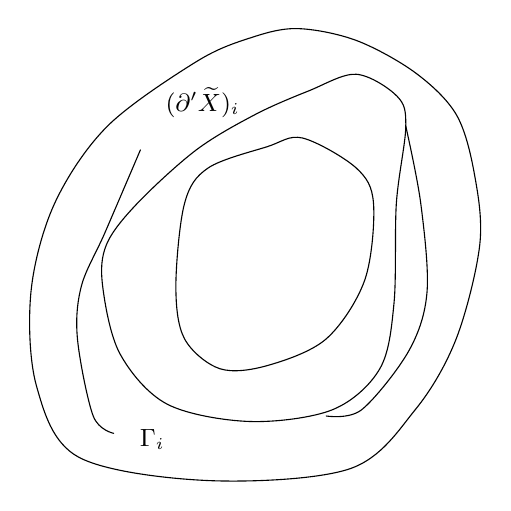
\begin{tikzpicture}[x=1mm,y=1mm,line cap=round,line join=round,font=\scriptsize]
\draw plot[smooth cycle, tension=0.55] coordinates {(52.5,-32.6) (57,-31.5) (63.8,-35.3) (66,-39.8) (64.9,-49.5) (60,-57) (52.5,-60.4) (46.5,-60.8) (42,-57) (40.9,-50.3) (42,-39.8) (45,-35.3)};
\draw plot[smooth cycle, tension=0.55] coordinates {(57.8,-25.5) (63.8,-23.4) (69,-26.2) (70.1,-30) (68.9,-39.8) (68.6,-52.5) (66.8,-60.8) (60.8,-66) (50.3,-67.5) (39.8,-65.3) (33.8,-58.9) (31.6,-50.3) (32.1,-45) (36,-39.8) (43.5,-33) (51,-28.5)};
\draw plot[smooth, tension=0.55] coordinates {(36.4,-33) (31.9,-43.5) (28.9,-50.3) (28.4,-57) (30.4,-66.8) (33,-69)};
\draw plot[smooth, tension=0.55] coordinates {(70.1,-30) (72,-39.8) (72.8,-51) (70.5,-58.5) (64.5,-66) (60,-66.8)};
\draw plot[smooth cycle, tension=0.55] coordinates {(56.3,-17.6) (63.8,-19.1) (71.3,-23.2) (76.5,-28.5) (78.8,-36) (79.5,-45) (76.5,-57) (71.3,-66) (63,-73.5) (45,-75) (28.5,-72) (23.2,-63) (22.5,-51) (25.5,-39.8) (32.2,-30) (43.5,-21.8) (50.3,-18.8)};
\node[inner sep=1pt] at (44.3,-27) {\small $(\partial'\widetilde X)_i$};
\node[inner sep=1pt] at (37.9,-69.8) {\small $\Gamma_i$};
\end{tikzpicture}
\end{document}
